\section{Implementation} % (fold)
\label{sec:implementation}

Using the requirements set forth in Section~\ref{sec:dvpns} we can compile a list of contemporary technologies that can meet them and provide \ac{dvpn}. The protocols considered had to meet \ref{lst:num} criteria:
\begin{inparaenum}[\itshape 1\upshape)]
	\item can provide Ethernet \acp{ppvpn} between multiple sites, and
	\item protocol stack must be supported in hardware at time of writing.
	\label{lst:num}
\end{inparaenum}

\subsection{\acs{spb}} % (fold)
\label{sub:spb}

\ac{spb} is an evolution of the original \acs{ieee} 802.1Q \ac{vlan} standard. \ac{vlan} tags have been in use in the networking world for a long time and provide decent separation in campus networks. However, when \ac{vlan}-tagging was done at the customer network, the carrier couldn't separate the traffic from different customers anymore. This resulted in 802.1Qad or Q-in-Q which added an S-\ac{vlan} tag to separate the client \acp{vlan} from the \ac{sp} \acp{vlan} in the backbone. This was usable for the Metro Ethernet networks for awhile but when \acp{sp} started providing this services to more and more customers, their backbone switches could not keep up with the clients \ac{mac} addresses.

To provide the required \acs{mac} scalability problem \ac{pbb} (802.1Qay or \ac{mac}-in-\ac{mac}) was introduced. It encapsulates the whole Ethernet frame on the edge of the carrier network and forwards the frame based on the Backbone-\ac{mac}, Backbone-\ac{vlan} and the I-SID. The I-SID is a Service Instance Identifier, which with 24 bits is able to supply the carrier with 16 million separate networks. The downside of \ac{pbb} remained one that is common to all Layer 2 forwarding protocols: the possibility of loops. Preventing them requires \ac{stp} which will disable links to get a loop-free network. Disadvantages of \ac{stp} include the relatively long convergence time and inefficient use of resources due to the disabled links. This final problem was solved by using \acs{isis} as a routing protocol to distributed the topology and creating \acp{spt} originating from each edge device. This is called \ac{spb} or 802.1aq.



% subsection spb (end)

\subsection{\acs{mpls}} % (fold)
\label{sub:mpls}

\ac{mpls} is known for its scalability and extensibility. Over the past decade additions have been made to the original specification to overcome a plethora of issues within carrier networks. This initially started with trying to implement fast forwarding in legacy switches using labels (or tags) at the start of the frame \cite{tag-switching}. When this issue became surmountable using new hardware, \ac{mpls} had already proven to be capable of transporting a wide arrange of protocols on the carrier backbone network, all the while also providing scalability, \ac{te} and \ac{qos} features to the operators.



\begin{figure}[!h]
	\centering
	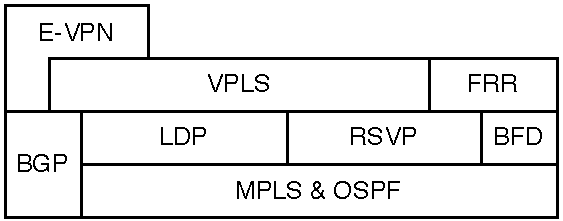
\includegraphics[width=7cm]{./includes/mpls-stack.pdf}
	\caption{Dependency stack of \ac{mpls}-related technologies.}
	\label{fig:mpls-stack}
\end{figure}

% subsection mpls (end)



\begin{table}[h]
	\centering
	\begin{tabular}{r|lll}
	 & \acs{spb} & \acs{mpls} & OpenFlow / \acs{sdn}\\
	\hline
	Tagging of VPN Traffic & \acs{pbb} & \acs{vpls} & \acs{pbb} / \acs{mpls}\\
	MAC Scalability & yes & yes & yes\\
	Topology Discovery & \acs{isis} & \acs{ospf} & application\\
	Path Provisioning & \acs{spt} & \acs{rsvp} / \acs{ldp} & application\\
	Traffic Engineering & limited & \acs{rsvp} & application\\
	\ac{ecmp} & limited & yes & yes, using Groups\\
	\ac{bum} limiting & dependent on \acs{hw} & dependent on \acs{hw} & yes, using Metering\\
	Exchange \acsp{cmac} & no & E-VPN (draft) & application\\
	Traffic Rate Limiting & dependent on \acs{hw} & dependent on \acs{hw} & yes, using Metering\\
	Fast Failover & no & \acs{frr} & yes, using Groups\\
	\acs{oam} & 802.1ag & \acs{lsp} Ping / \acs{bfd} & application\\
	\hline
	Forwarding Decision & \acs{pbb} tags & \acs{mpls} labels & flow entry \\
	\ac{bum} traffic handling & flood & flood & sent to controller\\
	\end{tabular}
	\caption{Required features and corresponding available technologies.}
	\label{tb:reqs}
\end{table}




Table of protocols

MPLS - tag of traffic
VPLS - encapsulates Ethernet frames
RSVP - distributes labels downstream / ecmp / te
LDP - distributes labels upstream / ecmp
OSPF - learns topology of network
BFD - provide connectivity checks

FRR depends on RSVP
RSVP depends on OSPF

LDP depends on VPLS
VPLS depends on RSVP and MPLS
RSVP depends on OSPF and MPLS

BGP depends on E-VPN
E-VPN depends VPLS
VPLS depends on RSVP
RSVP depends on OSPF and MPLS

depends all on MPLS forwarding plane

PBB - tag traffic
IS-IS - learns topology of network
SPB - ecmp / te

rate limiting, vendor specific

what can provide what function for DVPNs?

\subsection{Contemporary Technologies} % (fold)
\label{sub:contemporary_technologies}

% subsection contemporary_technologies (end)

\subsection{OpenFlow} % (fold)
\label{sub:openflow}

% subsection openflow (end)

% section implementation (end)